\chapter{Change-point detection for concentration data}\label{chp:4}

\minitoc

\clearpage

In this Chapter, we build a change-point detection algorithm specially adapted for concentration data. We will use that algorithm in the subsequent chapter to detect homogeneous temporal periods on which spatial statistical inferences will be possible. Several elements presented in Chapter \ref{chp:3} are used to build this method:  
\begin{itemize}
\item We use a parametric change-point detection, more precisely a maximum likelihood based method as described in Section \ref{chp:3:1}. The cost function $W$ is defined as the negative log likelihood of a distribution $Q$. The choice of $Q$ is motivated by the observation of the data, we mentioned in Chapter \ref{chp:2} that the distributions of concentrations were right skewed and presented long tails. Probability laws such as the Weibull are used for illustrations.  
%see Chapter \ref{chp:5} for an illustration on pesticide concentration data modelling.   
\item We use the PELT search method presented in Section \ref{chp:3:4} to obtain optimal solution to the change-point detection problem. Several penalty values $\beta$ are explored with the CROPS algorithm shown in Section \ref{chp:3:4}. The elbow method is applied when it is necessary to estimate an optimal number of change-points.   
\end{itemize}
We first describe the model integrating the censorship information in Section \ref{chp:4:1}. However, we do not know how much the censorship can affect a parametric change-point model. We provide a study of censoring effects in Section \ref{chp:4:2}. Furthermore, we need to devise an estimation procedure that is adapted to the observations of pesticide concentrations. The question sums up to detecting breaks in all dimensions of the parameters of $Q$ or not. We devise our estimation scheme in Section \ref{chp:4:3}. Finally, in Section \ref{chp:4:4}, we test our method against the \textit{Multrank} change-point method that can take into account the censoring in the data in its cost function. This method was introduced in Chapter \ref{chp:3}. 


\section{Generic model for censored data}\label{chp:4:1}

\subsection{Framework}

We present here the underlying parametric model we are using. We consider $\bm c = c_1,\dots,c_n$ which are realizations of independent real random variables $C_1,\dots,C_n$. The variables $C_i$ are recorded sequentially, and the recording times are not necessarily equidistant. Thus, the indices in $C_i$ are only indicators of the order of occurrence in the sample and not of the observation times. We suppose that there exist $K^*$ changes in the distribution of $\bm c$ happening at indices $0=\tau_0^*<\tau^*_1 <... < \tau^*_k <... < \tau^*_{K^*}<\tau^*_{K^*+1}=n$. Moreover, on the k-th segment, all random variables in the segment $C_{\tau^*_{k-1}+1:\tau^*_{k}}$ follow a distribution $Q$ with parameters defined by the vector $\theta^*_k\in\Theta$ with $\Theta\subset\mathbb{R}^P$. We denote $\bm{\theta^*} = (\theta^*_k)_{k=0}^{K^*}$. More formally, we have that:  
$$c_t \sim \sum_{k=0}^{K^*} f(.\vert\theta^*_k)\mathbbm{1}_{\tau^*_{k}+1\leq t \leq \tau^*_{k+1}},$$
$f$ being the density function of distribution $Q$ with respect to the Lebesgue measure on $\mathbb{R}$.  


The observations are subject to censoring. We focus on left-censorship because it is adapted for modelling concentration data but similar models can be created for right censorship or a mix of both. To each $c_i$ is associated a known censoring threshold $a_i \ge 0$. The resulting censored observations are defined by:  
\begin{equation}\label{chp:4:defy}
Y_i = \sup(C_i,a_i)
\end{equation}
Since the $C_i$ are independent and the $a_i$ are known deterministic values, the $Y_i$ are independent as well. The observations of $Y_i$ are denoted $y_i$. In this modelling, we can write the log-likelihood of a segment $y_{\tau^*_k+1:\tau^*_{k+1}}$ as:  
\begin{equation}\label{chp:4:loglik}
\mathcal{L}(y_{\tau^*_k+1:\tau^*_{k+1}},\theta^*_k) = \sum_{i = u}^v\log(f_{\theta^*_k}(y_i)) = \sum_{i = u}^v\log(F(y_i\vert\theta^*_k))\mathbbm{1}_{y_i=a_i}+\sum_{i = u}^v\log(f(y_i \vert\theta^*_k))\mathbbm{1}_{y_i>a_i},
\end{equation}
with $f_{\theta^*_k}$ being the density function of $Y_i$ for $i \in [\tau^*_k+1,\tau^*_{k+1}]$, $F(\vert\theta^*_k)$ being the cumulative distribution function (cdf) of $Q$. 

Note that if one needs to integrate right censorship into the likelihood, one should simply replace the $\sup$ in the definition \ref{chp:4:defy} by the $\inf$ of both quantities and cdf function $F$ by the survival function $S(t)=1-F(t)$. 


\subsection{Estimator choices and properties}

We define in this section the criterion and we choose the estimators of our method. 

We can define the cost function of  as:    
\begin{equation}\label{chp:4:costfunc}
W(y_{u:v}) = -\sup_{\theta\in\Theta}\{\sum_{i=u}^v\log(F(y_i,\theta))\mathbbm{1}_{y_i=a_i}+\sum_{i=u}^v\log(f(y_i,\theta))\mathbbm{1}_{y_i>a_i}\},
\end{equation}
with $F$ the cumulative distribution function (cdf) of $Q$.

Since we do not know the number of change point before hand, we opt for the penalized criterion defined in \ref{chp:3:4}. For a segmentation $\TT = \{\tau_1,...,\tau_K\}$ of a given signal $\bm y =\{y_1,\dots,y_n\}$, the penalised cost is given by: 
\begin{equation}\label{chp:4:pencost}
\CC(\bm y,\TT)=\sum_{i=0}^{K}  W(y_{\tau_i+1:\tau_{i+1}}) + KP\beta,
\end{equation}
where $P$ is the dimension of the parameters vector in the distribution $Q$ and $\beta > 0$ the penalty weight value. Gathering \ref{chp:4:costfunc} and \ref{chp:4:pencost}, this resulting estimator can be expressed as:  
\begin{equation}\label{chp:4:estim}
(\widehat{K},\widehat{\TT},\widehat{\bm \theta}) = \arg\min_{\TT,\bm \theta,K} \left(- \sum_{i=0}^{\lvert \TT \rvert}  \left\{\sum_{j=\tau_i+1}^{\tau_{i+1}}\log(F(y_j,\theta))\mathbbm{1}_{y_j=a_j}+\sum_{j=\tau_i+1}^{\tau_{i+1}}\log(f(y_j,\theta))\mathbbm{1}_{y_j>a_j}\right\}+\beta KP\right)
\end{equation}

We proceed to the estimation of its parameter using the maximum likelihood estimator $\widehat{\theta}_{u:v}$ on each segment $y_{u:v}$. It is defined by:
\begin{equation}\label{chp:4:emv}
\widehat{\theta}_{u:v} = \arg\max_{\theta \in \Theta}\mathcal{L}(y_{u:v},\theta)
\end{equation}

Furthermore, we assume the following on the model:  
\begin{itemize}
\item[\textbf{H1:}] $\Theta$ is compact and there exists $\Delta_{\bm \theta}^{\star}>0$ such that $\vert \theta_{k+1}^{\star}-\theta_{k}^{\star}\vert > \Delta_{\bm \theta}^{\star}$, for all $k=0,...,K^{\star}$.
\item[\textbf{H2:}] There exists $\Delta_{\bm \tau}^*>0$ such that $\vert \tau_{k}^{\star}-\tau_{k-1}^{\star}\vert > \Delta^*_{\bm \tau}$, for all $k=1,...,K^{\star}$.
\item[\textbf{H3:}]  There exists a positive integer $K_{max}$ such that the maximum number of regimes $\frac{n}{\Delta^*_{\bm \tau}}$ satisfies $K_{\max} \geq \frac{n}{\Delta^*_{\bm \tau}}$. 
\item[\textbf{H4:}] The penalty value is dependant of $n$. It can be written $\beta_{n}$ and verifies $\beta_{n}\xrightarrow[n\rightarrow \infty]{} \infty$ and $\frac{\beta_{n}}{n}\xrightarrow[n\rightarrow \infty]{} 0$.
\end{itemize}

These are standard hypotheses that can be found in \cite{Lavielle1997} or \cite{He2010}. Hypothesis \textbf{H1} mainly aims at ensuring sufficient conditions for the identifiability of the model, by imposing a minimum gap between two consecutive $\theta$'s. 

Hypothesis \textbf{H2} checks that each regime contains sufficient data for obtaining reliable estimates for the $\theta$'s and Hypothesis \textbf{H3} states the number of regimes is bounded from above.  

Hypothesis \textbf{H4} is verified by a large range of penalties including the BIC \citep{YAO1988181}. 

We formulate an additional hypothesis \textbf{H5}, which is also the strongest one. 
\begin{itemize}
\item[\textbf{H5:}] Change-point locations are independent of the scale and frequency at which the data is sampled
\end{itemize}
This hypothesis will also allow us to derive the asymptotic behaviour of the estimator, when the sample size is sufficiently large. One should note here that a larger sample means a finer scale for sampling the data and not an extension of the period of observation. 

Note that in practice, for environmental data with scarce and irregular sampling, this hypothesis is hard to verify.
However, we may suppose that the change-points occurring in concentration data are linked with the farming activities and the phyto-pharmaceutical uses, regardless of the sampling rate. 

Under these assumptions, we know that the maximum likelihood estimator computed in Equation \ref{chp:4:estim} is weakly consistent \citep{Lavielle1997}. \begin{equation}
(\widehat{K},\widehat{\mathcal{T}},\widehat{\theta}) \xrightarrow[n\to+\infty]{\mathbb{P}} (K^*,\mathcal{T}^*,\theta^*)
\end{equation}
Elements of proof are provided in Appendix \ref{app:chap4:1}. 

%However, even when \textbf{H1} holds, censorship may cause identifiability issues that will be handled in Section \ref{chp:4:2}.
%we show in Section  that censorship could cause additional identifiability problems that will require specific .  
%implies that . 
%The sampling quality (size and regularity of   being one of the main problem of the data we are working with, it would be hard to verify asymptotic properties. 

\subsection{Estimation procedure}

\subsubsection{Estimation of parameters for a single homogeneous segment}

For a given $y_{u:v}$, one should be able to properly compute $\widehat{\theta}_{u:v}$. as the estimate of the parameter of $Q$. It is impossible to obtain a explicit formula of $\widehat{\theta}_{u:v}$ when there are censored observations in the sample. Still, one derives the estimator value through a numerical optimisation procedure. The Newton-Raphson method was used to search for the zeros of the first derivative of the cost function.  

For some choices of $Q$, checking that the cost function is strictly convex is not always easy. However, we can still show that the cost is locally convex and has a unique minimum by studying its variations. This implies a careful choice in the parameter initialization value of the Newton-Raphson method to obtain convergence of $\widehat{\theta}_{u:v}$. Appendix \ref{app:chap4:2} provides experiments on the initialization of the Newton-Raphson method. 

\subsubsection{Estimation procedure for $K^*$, $\mathcal{T}^*$ and $\theta^*$}

The estimation procedure aims at maximising the penalised log-likelihood in Equation \ref{chp:4:pencost}. The optimisation procedure implies finding both the best partitioning of the data as defined by $\widehat{K}$ and $\widehat{\mathcal{T}}$, as well as the estimates for the parameters of the distribution $Q$ within each segment, $\widehat{\theta}$. 

We proceed using the PELT algorithm (see Section \ref{chp:3:4}). In practice, we use the following value for the cost function to evaluate a given segment $y_{u:v}$:
\begin{equation}
W(y_{u:v},\widehat{\theta}_{u:v}) = \sum_{i=u}^v\log(F(y_i,\widehat{\theta}_{u:v}))\mathbbm{1}_{y_i=a_i}+\sum_{i=u}^v\log(f(y_i,\widehat{\theta}_{u:v}))\mathbbm{1}_{y_i>a_i},
\end{equation} 
where $\widehat{\theta}_{u:v}$ is the output of the Newton-Raphson method, trained on segment $y_{u:v}$. 

\subsubsection{Selecting the optimal number of changes}

We use the CROPS algorithm (see Section \ref{chp:3:4}) to select the optimal number of change points in the signal. The penalty range selected investigated is derived from the BIC criterion formula \citep{YAO1988181}.  
Note that this choice verifies assumption \textbf{H4}. In change point detection, the BIC penalty can be written as: 
\begin{equation}
\beta_{BIC} = \frac{P\log(n)}{2},
\end{equation}
with $P$ the dimension of the parameters $\theta$ and $n$ the length of signal $\bm y$. The penalty range value explored in this thesis writes under the form: 
\begin{equation}
[\beta_{min},\beta_{max}] = [\frac{\beta_{BIC}}{j},\beta_{BIC}\times j],
\end{equation}
with $j\in\mathbb{N}$. Hence, our penalty range is calibrated accordingly to Hypothesis \textbf{H4} because $\beta_{min}$ and $\beta_{max}$ also verifies its conditions.  

Once we run CROPS, we obtain some penalty values $\{\beta_{min},\dots,\beta_{max}\}$. Since each of these penalty values is associated to a cost segmentation and a number of change points, we can perform the elbow method heuristic (see Algorithm \ref{chp:3:algoelbow}) on the curve of the segmentation costs in function of the number of changes. An optimal number of break points and the associated procedure are thus selected with this procedure.
%Let us mention here that Algorithm 1 relies on a series of hyper-parameters which ought to be tuned: the precision threshold and the maximum number of iterations in the Newton-Raphson step, the initial values for the l’s in Newton-Raphson step also, and the minimum number of observations between two consecutive change-points. In the experiments we performed, the initial values for the l’s were set as the inverse of the observed average value in the respective segment.
%the thus guaranteeing the unicity of the maximum likelihood estimate.
%\rightarrow_{n\to+\infty}^{\mathbb{P}}
%Although these hypotheses guarantee the convergence of estimates in the classical framework (e.g. just as in \cite{Lavielle1997}), we need to examine the effects of censoring in our method, which is a factor that places us out of the classical framework.

Let us now study the effect of censorship on our procedure.

\section{Censoring effects}\label{chp:4:2}

%We are interested in the effects of censorship on two main aspects: 
%\begin{itemize}
%\item The quality of the estimation of the parameters $\bm \theta$ of $Q$ on a fixed segment. 
%\item The implication it can have on the search method PELT and how to adapt it if this is the case. 
%\end{itemize} 
%
%\subsection{On the parameter estimation for one segment}\label{chp:4:cens_seg}
%On the change point detection method

The censorship can pose problems in the practical implementation of the procedure developed in Section \ref{chp:4:1}. In particular, issues can be encountered when estimating the parameter of a fully censored segment with Newton-Raphson. Illustrating examples are provided in this section with $Q$ set as the exponential distribution.

\subsection{Practical problem encountered with censoring}\label{chp:4:cens_seg}

%The cost functions need to be twice differentiable in $\theta$. We search for the zeros of the first derivative of the cost function in order to find a global minimum. 
%Checking that the second derivative is strictly positive in presence of censored data, thus guaranteeing the unicity of the maximum likelihood estimate, can prove to be a difficult task as it is not always the case for all distributions $Q$. 
%We provide an example of such a case in Appendix \ref{app:chap4:2} where we prove the existence of a global minimum without having the global convexity of the first derivate. 


In general, an explicit formula for the maximum likelihood estimator (MLE) is not available in presence of censored data, leading to the use of numerical methods for its computation. The Newton-Raphson method was used on each segment to compute the MLE estimate of $\theta$. 

Specifically, the case where all data in the segment $y_{u:v}$ are censored is problematic. Looking at the analytical likelihood formula, we find that the $\theta$ realising the minimum of the cost function is still unique, but tends toward infinity. In this case the cost tends to zero. We illustrate in Figure \ref{fig:onlycens} with $Q$ set as an exponential distribution. 
For a given segment $y_{u:v}$ where all observations are censored and under a censorship threshold $a$ we have that: 
\begin{equation} \label{chp:4:costex}
W(y_{u:v}) = -\sup_{\theta \in \Theta}(v-u)\log(1-\exp(-\theta a)) 
\end{equation}
This cost is always positive and decreasing to 0 when $\theta$  goes to infinity. 
\begin{figure}[ht]
    \centering
    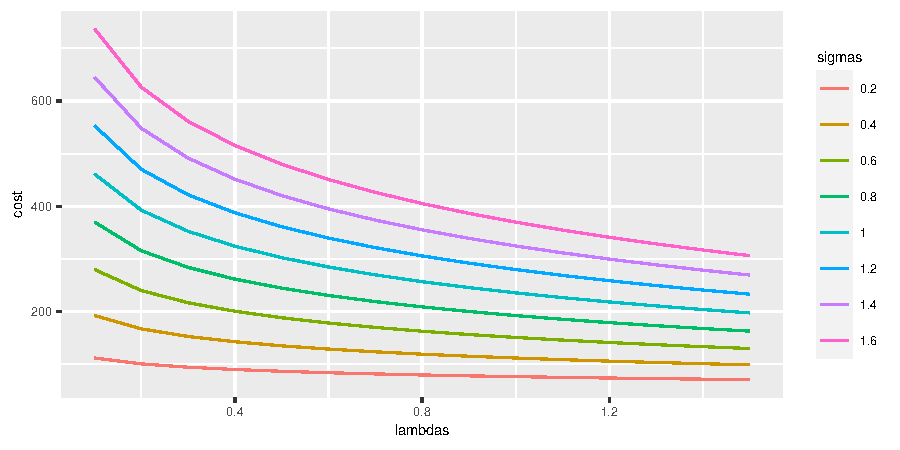
\includegraphics{figs/Chap4/only_cens.pdf}
    \caption{Plot of the cost function values against $\theta$ values when all observations are censored. It is represented for an exponential distribution. The sample consists in 100 values of censored observations to a threshold $a = 0.05$.}
    \label{fig:onlycens}
\end{figure}
%We show in the next part why it could be problematic to have fully censored segments in the search method and how we chose to deal with it. 
%\subsection{On the change point detection method}

We made the assumption that the support $\Theta$ of the segments parameters is a compact of $\mathbb{R}$ in Section \ref{chp:4:1} . This corresponds to hypothesis \textbf{H1}. Hence, we need to decide of an upper bound for $\Theta$. We show in the next section how we proceed. 

%This means that there is an upper bound $\theta_{max}$ such that $\theta\geq\theta_{max}$ for all $\theta$.
%The case of fully censored segments are questioning the identifiability of the change-point detection method. This assumption is summarized in hypothesis \textbf{H1} of Section \ref{chp:4:1}.  
%\citep{Lavielle1997} 
%for the segment parameters is the following:   
%\begin{itemize}
%\item[] $\Theta$ is compact and there exists $\Delta_{\bm \theta}^{\star}>0$ such that $\vert \theta_{k+1}^{\star}-\theta_{k}^{\star}\vert > \Delta_{\bm \theta}^{\star}$, for all $k=0,...,K^{\star}$. 
%\end{itemize}

\subsection{Introduction of an upper bound parameter on $\theta$}

%If that is the case $\Theta$ is not compact.
We have seen in Section \ref{chp:4:cens_seg} that, for the exponential distribution example, the optimal $\theta$ tends to infinity. To solve this practical problem, we introduce an additional parameter $\theta_{max}$ in our implementation such that $\theta$ is constrained to the interval $[0,\theta_{max}]$ which is a compact part of $\mathbbm{R}$. 

A new problem arises from this modelling choice. The value of $\theta_{max}$ must be chosen carefully. We must ensure that $\theta_{max}> \theta^*_k,$ for all $k \in \{0,\dots,K^*\}$. If it is not the case, the identifiability problem remains. For two $\theta^*_i$ and $\theta^*_j$  greater than $\theta_{max}$, their estimates will be set to $\theta_{max}$ and thus no segment identifiability will be possible. 

In order to avoid such problems, the value of $\theta_{max}$ is set according to the worst censoring case scenario possible. More precisely, we assume no change-point occurred in $\bm y$ and that all observations are distributed according to $Q$ with parameter $\theta_{max}$. We set $\theta_{max}$ to the value such that: 
\begin{equation}
F(\min(\bm y),\theta_{max})^n = \alpha,
\end{equation}
with $\alpha$ being a desired percentage of censorship. In practice, we decide to set $\alpha$ to $95\%$. This corresponds to the scenario where there is a $95\%$ chance that $n$ observations generated from the distribution $Q$ with parameter $\theta_{max}$ are left-censored and under the threshold $a = \min(\bm y)$. 
% $95\%$ of the observation in $\bm y$ would be censored and would be lesser to the smallest censoring threshold value. 

We provide a practical example with the exponential distribution. We simulate a signal $\bm y$ of size $n = 200$ that is a realization of exponential distributions of parameters $\theta^*_0 = 1$ for $y_{1:100}$ and $\theta^*_1 = 4$ for $y_{101:200}$. The censoring level is set to the median of $\bm y$ so that 50$\%$ of the signal is censored. We illustrates $\bm y$ in Figure \ref{fig:theta_max}. We set $\theta_{max}$ choosing with $\alpha = 95\%$. We have that $\theta_{max} = \frac{-\log(1-\alpha^{1/n})}{\min(\bm y)}$. In our numerical example, $\theta_{max} = 24.68$, which is greater than $\theta_0$ and $\theta_1$.

\begin{figure}[ht]
    \centering
    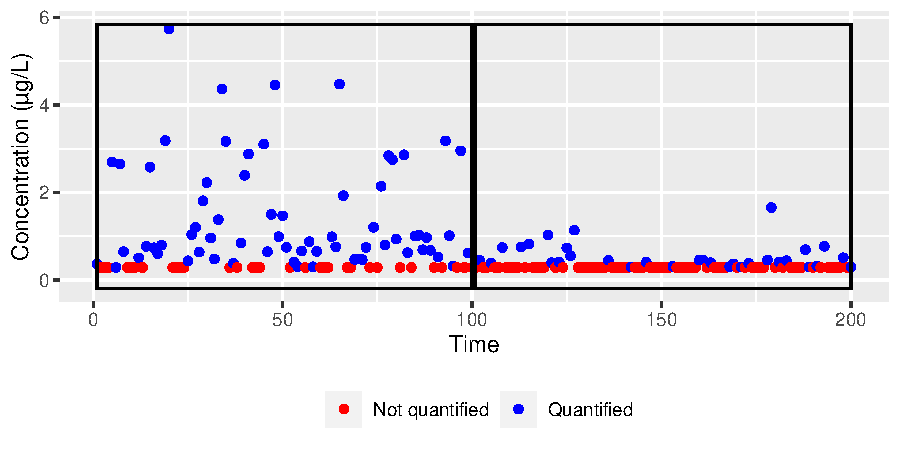
\includegraphics{figs/Chap4/theta_max_ex.pdf}
    \caption{Example of simulated signal $\bm y$ distributed according exponential distributions. The two segments are drawn with black rectangles. $\theta^*_0 = 1$ in the left segment, $\theta^*_1 = 4$ in the right one and the censoring threshold $a = 0.28$ in both segments}
    \label{fig:theta_max}
\end{figure}

Note that other ways to tackle this problem are possible. The modification of the pruning rule \ref{chp:3:pruning} used in PELT can also be investigated. For example, one could decide to systematically discard all potential change-point indices $\tau \in \{u,\dots,v\}$ when evaluating a fully censored segment $y_{u:v}$.  

\section{Multi-dimensional parameter estimation}\label{chp:4:3}

%When $\theta$ is a parameter vector of dimension $P>1$, a common strategy is to opt for simultaneous changes detection in all $P$ parameters simultaneously. This implies detecting changes in different properties of $\bm y$. In practice, it depends on what parameters are optimized in the cost function. The optimization can still be performed with numerical methods (such as Newton-Raphson) on all dimensions of $\theta$ simultaneously. Plugging an estimator of the parameters vector in a cost function defined in Equation \ref{chp:4:costfunc} would results in
%Using a MLE estimators of all $P$ parameters as the supremum in \ref{chp:4:costfunc} provide a cost function that detects changes occurring in any of the parameters.  


Two separate cases can occur when the parameter $\theta$ is a vector of dimension $P > 1$.  

We can distinct the first case where the detection is made in all dimension of the parameter vector. In that case, this implies detecting changes in different properties of $\bm y$ simultaneously (mean and variance for example). In practice, it is still possible to compute the maximum likelihood estimator in Equation \ref{chp:4:emv} with numerical methods (such as Newton-Raphson for example). The problem with such a modelling choice resides in the number of data needed in a segment to estimate all parameters. The number of observations must be more important to have a valid statistical estimation when the number of parameters to estimate is high.  

In the second case, some dimension of the parameters vector $\theta$ are supposed to be constant over time. In this setting, we can either suppose that the fixed parameters are known in which case the change point detection procedure can be done with a correct cost function. For example a quadratic loss function is practical for detecting changes in the mean of a signal without estimating the variance (that is supposed to be fixed) \citep{Fearnhead2018a}. 

In practice, this modelling choice can be justified if some parameters values are supposed to control the intrinsic diffusion properties of a chemical substance in the environment. Then, these parameters should be invariant in time. The parameters changing at each segment could represent different intensities in the substance's use in time for example. 

An example with $Q$ set as a Weibull distribution is provided in Figure \ref{fig:param_ex}. 
\begin{figure}[ht]
    \centering
    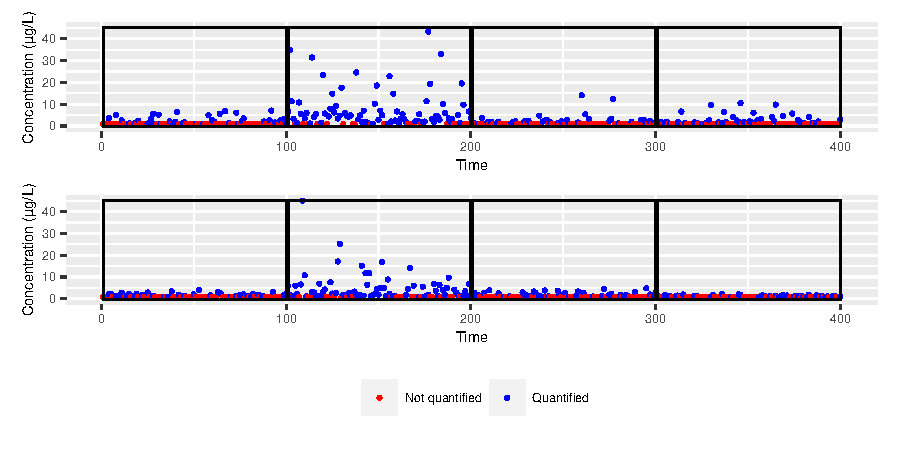
\includegraphics{figs/Chap4/param_ex.pdf}
    \caption{Example of simulated signal $\bm y$ distributed according Weibull distributions with $(\lambda,\sigma)$ as the scale and shape parameters. The segments are drawn with black rectangles. \\ 
\textbf{Upper signal:} The associated parameters to each segment are $\theta^*_{0,.} = (\lambda^*_0,\sigma^*_0) = (1,1)$, $\theta^*_{1,.} = (\lambda^*_1,\sigma^*_1) = (3,0.7)$, $\theta^*_{2,.} = (\lambda^*_2,\sigma^*_2) = (1,0.7)$, $\theta^*_{3,.} = (\lambda^*_3,\sigma^*_3) = (1,2)$ and the censoring threshold $a = 0.86$ in all segments.\\
\textbf{Lower signal:} The associated parameters to each segment are $\theta^*_{0,.} = (\lambda^*_0,\sigma^*) = (1,0.7)$, $\theta^*_{1,.} = (\lambda^*_1,\sigma^*) = (5,0.7)$, $\theta^*_{2,.} = (\lambda^*_2,\sigma^*) = (0.7,0.7)$, $\theta^*_{3,.} = (\lambda^*_3,\sigma^*) = (1,0.7)$ and the censoring threshold $a = 0.89$ in all segments.}
    \label{fig:param_ex}
\end{figure}

Note that all the estimation schemes we mentioned rely on the fact the criterion to be optimized is additive. other ways to estimate changes in a signal exist without this property like MCMC algorithms \citep{Lavielle2001} or genetic algorithms but they are not in the scope of this thesis.  


\subsection{Estimators of a segmentation with some fixed parameters}

We discuss here the procedure for the parameters estimates proposed in \ref{chp:4:estim}. When $\theta^* \in \mathbb{R}^P$ with $P > 1$, several optimization strategies are possible. We use the following notations in this section: 
\begin{itemize}
\item $\bm \theta_{.,m} = (\theta_{0,m},\dots,\theta_{K,m})$ is the m-th dimension of the parameters vector of each segment $k$.
\item $\bm \theta_{k,.} = (\theta_{k,1},\dots,\theta_{k,P})$ is the parameters vector of the k-th segment.
\item $\theta_{k,m}$ is the m-th dimension of the parameters vector of the k-th segment.
\end{itemize}

We propose a different estimation strategy. We are interested in models where changes occur only in some dimension $\bm\theta^*_{.,m}$. We denote $\mathcal{M} \subset \{1,\dots,P\}$ the set of indices of dimensions where the changes occur and $\overline{\mathcal{M}}$ the complementary set. Figure \ref{fig:param_ex} provides an illustration of signal $\bm y$ simulated from these assumptions. The parameters $(\bm\theta^*_{.,m})_{m \in \overline{\mathcal{M}}}$ are supposed to be fixed throughout the signal $\bm y$. In that setting, the estimation procedure differs from Equation \ref{chp:4:estim} and we can deduce its expression: 
    
\begin{dmath}\label{chp:4:estimproc}
(\widehat{K},\widehat{\TT},\widehat{\theta}_{.,m\in\mathcal{M}},\widehat{\theta}_{.,m\in\overline{\mathcal{M}}}) = \arg\min_{K,\TT,\bm \theta_{.,m\in\mathcal{M}}}\bigg[\arg\min_{\theta_{.,m\in\overline{\mathcal{M}}}}\bigg\{ - \sum_{i=0}^{\lvert \TT \rvert}  \left(\sum_{j=\tau_i+1}^{\tau_{i+1}}\log(F(y_j,\theta))\mathbbm{1}_{y_j=a_j}+\sum_{j=\tau_i+1}^{\tau_{i+1}}\log(f(y_j,\theta))\mathbbm{1}_{y_j>a_j}\right)\bigg\}+\beta KP \bigg]
\end{dmath}

From \ref{chp:4:estimproc}, we can design a two-step iterative estimation strategy.

\subsection{Estimation procedure}

We describe the practical implementation of the estimation Equation \ref{chp:4:estimproc}. We choose to proceed with a two steps iterative algorithm. 
The two steps of each iteration can be described as:
\begin{enumerate}
\item Compute the MLE $\widehat{\bm\theta}_{{.,m\in\overline{\mathcal{M}}}}$ with fixed $\widehat{\TT}$ and $\widehat{\theta}_{.,m\in\mathcal{M}}$ with any optimization method that handles censored data. We use \texttt{R} package developed in \cite{delignette2015} in our procedure.  
\item Run the change-point procedure of to estimate $\widehat{\TT}$ and $\widehat{\theta}_{.,m\in\mathcal{M}}$ using the values of $\widehat{\bm\theta}_{{.,m\in\overline{\mathcal{M}}}}$.
\end{enumerate} 

In the second step of an iteration, we compute a new segmentation from the value of $\widehat{\bm\theta}_{{.,m\in\overline{\mathcal{M}}}}$ using a similar procedure as the one described in Section \ref{chp:4:1}. More precisely, we run PELT several times on penalty values included in a range $[\beta_{min},\beta_{max]}$. Once several results of segmentation are acquired, $\widehat{\TT}$ and $\widehat{\theta}_{.,m\in\mathcal{M}}$ are chosen using the elbow heuristic as proposed in Section \ref{chp:3:3}.   

The difference is that we do not use the CROPS algorithm to explore the penalty range. Instead, we use a penalty grid $(\beta_0,\dots,\beta_q,\dots,\beta_{B})$ where $\beta_0<\dots<\beta_{q}<\dots<\beta_{B}$ are evenly spaced. This can be justified by the fact that the penalty values explored by CROPS would change at each iteration. We want to be sure that the selection step made with the elbow heuristic is made on segmentations issued from the same penalty values. 
%we want to be able to compare each set of segmentations at each iteration. Since ,  

%the estimated segmentation $\widehat{\TT}$ and the fitted parameters on its segments $\widehat{\theta}_{.,m\in\mathcal{M}}$ are obtained by applying the PELT procedure \citep{Killick2012}. PELT is run several times on a penalty grid $(\beta_0,\dots,\beta_q,\dots,\beta_{B})$ where $\beta_0<\dots<\beta_{q}<\dots<\beta_{B}$ are evenly spaced. We obtain $B$ segmentations of $\bm{y}$. Eventually, the optimal penalty value for this step is selected using an elbow rule heuristic as proposed in Section \ref{chp:3:3}.

The initialization is an important part of this procedure. We would like the initial estimate of the fixed parameters to be close to $\bm\theta^*_{{.,m\in\overline{\mathcal{M}}}}$ to ensure the convergence of the procedure. In order to do so, we initialise $\widehat{\bm\theta}$ assuming no change-point occurred in $\bm y$.  More formally, we compute: 
\begin{equation}\label{chp:4:init}
\widehat{\bm\theta} = \arg\min_{\theta}\bigg\{ - \left(\sum_{j=1}^{n}\log(F(y_j,\theta))\mathbbm{1}_{y_j=a_j}+\sum_{j=1}^{n}\log(f(y_j,\theta))\mathbbm{1}_{y_j>a_j}\right)\bigg\}
\end{equation}   

We proceed using the MLE estimator for all parameters in $\bm \theta$, which implies using iterative methods again as stated in \cite{cohen1965maximum}. We choose the initial values as the $\widehat{\bm\theta}_{.,m}$ such that $m\in\overline{\mathcal{M}}$. 

It can be noted straight away that the value of $\widehat{\bm\theta}_{.,m\in\mathcal{M}}$ will be discarded since it was computed from a model that goes in direct contradiction with the assumption in \ref{chp:4:1} that they were change-points in the signal $\bm y$. 

We show the efficiency of this procedure in Appendix \ref{app:chap4:3}.  

We use this procedure estimation in Chapter \ref{chp:5}. We justify this choice with the observation of real data. We compare the efficiency of our method a state-of-the-art in the next section.

\section{Simulation study}\label{chp:4:4}

We test our method on simulated data and compare it with the \textit{Multrank} method \cite{lung2015}. This section aims at two objectives. First, we want to calibrate the parameters of our method to ensure good efficiency. Then, we want to test if that calibration really leads to better change-point results.  

\subsection{Testing the detecting capacity}

In section \ref{chp:2:2}, the PELT Algorithm \ref{chp:3:algopelt} introduces a minimal segment length $n_{min}$. We lead some simulation tests to calibrate its value. We need to identify $n_{min}$ so that the cost function defined in \ref{chp:4:costfunc} has sufficient data to detect a change between two segments with different parameters.
%make the difference between segments on which the parameters differ. 

This task can be viewed as a classification one. We want to know if our method is able to classify correctly signals that have a change point or not. Since we use a parametric inference (see Section \ref{chp:4:1}), we use the log likelihood ratio test to assess the presence of a change-point. This is a very common test used in change-point that can be found in. The statistics of the likelihood ratio test are calculated on several simulated signals and and the ROC curves \citep{Fawcett2006} are derived from it. We compute the corresponding areas under the curve (AUC) to assess the ability to detect change-points of our method. A comparison of our method is made with the \textit{MultRank} method that is based on non parametric inference that we presented in Section \ref{chp:3:1}. We will use this comparison to calibrate our method performance.  

The simulation procedure for the calibration of $n_{min}$ is the following. We use the Weibull distribution for the distribution $Q$. We test several configurations with different censoring levels $\alpha = (5\%,25\%,50\%,75\%,95\%)$. It is a global censoring level, meaning that for a given signal $\bm y$, $\alpha\%$ of the data is censored. The detection methods are run with different values of minimal segment size $n_{min} = (5,10,25,50,75)$. For each configuration, we simulate $M = 1000$ signals of size $n = 200$ among which half of them present a change point in position 100. The parameters of signals with a change-point are $(\sigma = 0.5,\lambda^*_0 = 1)$ on the first segment and $(\sigma = 0.5,\lambda^*_1 = 3)$ on the second. The parameters associated to signals with no change-point are $(\sigma = 0.5,\lambda = 1)$. We compute the AUC on these $M$ signals. The results are illustrated in Figure \ref{fig:sim_minseg}.      

\begin{figure}[ht]
\centering
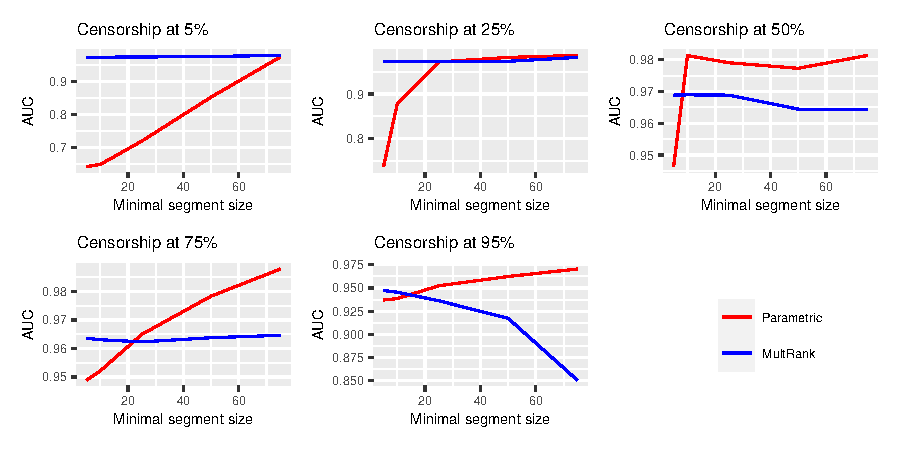
\includegraphics{figs/Chap4/sim_minseg.pdf}
\caption{Choice of the minimal segment length: simulation results. Our method performance is Illustrated with the red dots, the \textit{Multrank} method is drawn in blue.}
\label{fig:sim_minseg}
\end{figure}

From the results of Figure \ref{fig:sim_minseg}, three comments can be made:  
\begin{itemize}
\item Both methods are efficient in their abilities to detect change-points in signal. The AUC are above 0.9 (except for the parametric method in a highly censored configuration with a low value minimal segment size). That make them both good classifiers. 
\item The performance of the parametric method increases with the minimum segment length. 
\item The more the censoring levels increase, the more data is needed in the minimal segment length of the parametric method to outclass the non parametric method. 
\end{itemize}
From this study, we can conclude that when working with real data, we should get the censoring level information information in order to calibrate the minimal segment length of the parametric method.  

\subsection{Testing the precision of the detection method}

We want to compare the performance of the change-point detection with the Multrank method developed in \cite{lung2015} since both methods are adapted to censored data. We examine the capacity to estimate the correct number of breaks in a signal and the precision of the change-point position. This section is illustrated using the Weibull distribution.   

The experimental framework is as follows: 
    \begin{enumerate}
        \item we simulate $N=100$ samples $(x_1,...,x_n)$ of size $n=400$  following a left-censored Weibull distribution with $\alpha\%$ of censored data. We made tests for the different censorship rates $\alpha = (25,50,75,95)$. The shape parameter of the Weibull distribution is assumed to be known and set to $\sigma=0.5$. The scaling parameters $\bm{\lambda^\star}$ have $K^\star=4$ breaks at positions $p^\star_1 = 80$, $p^\star_2 = 160$, $p^\star_3 = 240$ and $p^\star_4 = 320$ and take the values $\bm{\lambda^\star}=(\lambda^\star_1 = 1, \lambda^\star_2 = 4, \lambda^\star_3 = 0.5, \lambda^\star_4 = 5, \lambda^\star_5 = 1)$. An example of a sample simulated in this way is shown in Figure \ref{fig:ex_sim}.
        \item For each of the $N$ samples, we perform the parametric change-point detection and the Multrank methods. For each sample, we obtain the estimated number of breaks $\hat K_{param}$ and $\hat K_{multrank}$ and their position $(\hat{p}_{k,param})_{k = 1}^{\hat K_{param}}$ (respectively $(\hat{p}_{k,multrank})_{k = 1}^{\hat K_{multrank}}$).
        \item for both methods, we count the number of samples among the $N$ for which the correct number of breaks has been estimated (e.g. $\hat K_{param} = K^\star$). Also, for each of the samples for which the estimate of $K^\star$ is correct, we make an histogram of the change-points position. 
    \end{enumerate}
Since $K$ is not known, we proceed as follows for each method to estimate it:
    \begin{itemize}
        \item For the parametric method: we use the algorithm CROPS, algorithm to scan a continuous range of penalty values $[\beta_{min},\beta_{max}]$. We obtain a set of $B$ values $(\hat \beta_1,...,\beta_B)$ and the optimal segmentations associated with these penalty values. We then plot the cost of the segmentations as a function of the number of breaks. We choose the optimal penalty using a elbow heuristic. This procedure is described in \cite{haynes2014}. The choice of $\beta_{min}$ and $\beta_{max}$ is inspired from linear penalties like the BIC criterion \cite{YAO1988181}. Note that when using the BIC penalty in change point detection, the penalty term written in section \ref{chp:4:1} becomes : $\beta_n = \frac{P}{2}\log(n) = \frac{1}{2}\log(n)$, where $P$ is the number of dimensions of the parameter. More precisely, we took a wide interval of penalty values defined by $\beta_{min} = \frac{\log(n)}{10}$ and $\beta_{max} = 5\log(n)$.
        \item For the non parametric \textit{Multrank} method, we compute using the optimal segmentation search method presented in Algorithm \ref{chp:3:algoopt} for $k$ breaks, where $k$ ranges from $1$ to $K_{max}$. For each of these segmentations, we can compute the cost of the segmentations using the cost function in \ref{chp2:costfuncnp}. As in the parametric method, we represent the costs as a function of $k$, and we determine the number of estimated breaks by an elbow heuristic. Here, $K_{max}$ is fixed at $2*K^\star = 8$.
    \end{itemize}
The results of the simulations are shown in Table \ref{tab:simcomp} and in Figure \ref{fig:prec_sim}. It can be seen that in the ideal scenario, where the data are indeed distributed according to a left-censored Weibull distribution, the parametric method performs better both in detecting the correct number of breaks and in accurately estimating their position. However, this performance decreases as the censoring rate increases.

\begin{figure}[ht]
    \centering
    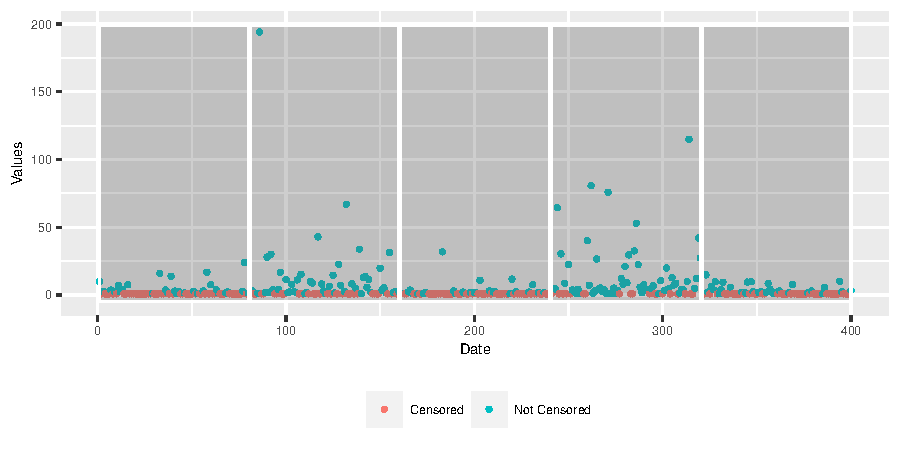
\includegraphics{figs/Chap4/Ex_sim.pdf}
    \caption{Example of simulated signal with $(\lambda_1 = 1, \lambda_2 = 4, \lambda_3 = 0.5, \lambda_4 = 5, \lambda_5 = 1)$, $\sigma = 0.5 $, $n = 400$, $K = 4$, $(p_1 = 80,p_2 = 160,p_3 = 240,p_4 = 320)$ and $\alpha = 50\%$.}
    \label{fig:ex_sim}
\end{figure}

\begin{table}[ht]
\centering
\begin{tabular}{|r|r|r|}
  \hline
   $\alpha(\%)$  & Parametric method & MultRank \\ 
  \hline
 25 &  84 &  58 \\ 
 50 &  80 &  63 \\ 
 75 &  87 &  68 \\ 
 95 &  65 &  10 \\ 
   \hline
\end{tabular}
\caption{Number of correct estimations of $K$ over $N=100$ samples for both methods for different $\alpha\%$ censorship rates.}
\label{tab:simcomp}
\end{table}

\begin{figure}[ht]
    \centering
    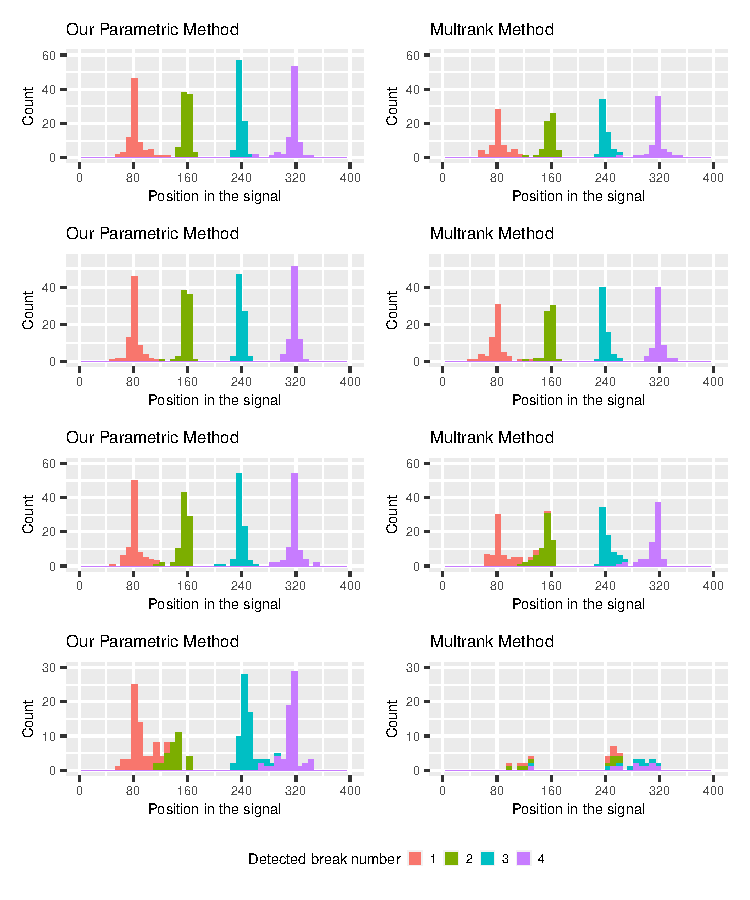
\includegraphics{figs/Chap4/detect_comp.pdf}
    \caption{Precision of the estimated change-points for both methods.}
    \label{fig:prec_sim}
\end{figure}

\clearpage

\section{Chapter summary}

This Chapter designs and tests an adapted change-point detection method for concentration data. The censorship is handled by the cost function choice in Section \ref{chp:4:2}. More precisely, using a parametric approach as presented in Chapter \ref{chp:3}, the likelihood is adapted to distinguish cases were a measure is censored or not. The censorship becomes critical for computing the maximum likelihood estimate of a segment when all observations are censored. This could cause issues in the identifiability of segments parameters which would compromise the detection method capacity. However, one way to circumvent this problem is to introduce a new regularization parameter in the detection that is a maximum value for the parameter value. The estimation strategy is also discussed in this Section \ref{chp:4:3}. An estimation scheme where some parameters dimension are fixed in time and other can vary across segments is devised. Experiments of Section \ref{chp:4:4} ensure that, if enough data is available to evaluate a segment, the parametric method performs decently and can outclass a suited non parametric method for censored data. 

Chapter \ref{chp:5} combines the results of temporal change-point detection using the parametric method developed in this Chapter with statistical methods to deal with the spatial heterogeneity. The obtention of homogeneous temporal sub signal in the concentrations values provides the temporal context in which the spatial analysis is conducted. In particular, in this homogeneous temporal setting, it is interesting to look for geographical areas that had concentration values that differ from others. Constructing these areas and comparing them is the main topic of Chapter \ref{chp:5}. Chapter \ref{chp:6} is the presentation of the results of Chapter \ref{chp:5} and \ref{chp:4} applied to the concentration data of substance. The results of all methods are all gathered using an interactive presentation tool.     

       

 